%\documentclass[dvipdfmx]{beamer}
\documentclass[dvipdfmx,final,t,10pt]{beamer}
\usepackage[orientation=portrait,size=a4,scale=1.4]{beamerposter}%縦 : orientation=portrait, 横 : orientation=landscape
\usepackage{here, amsmath, latexsym, amssymb, bm, ascmac, mathtools, multicol, tcolorbox}
\usepackage{listings}
%\usepackage{luatexja}
%\usepackage{luatexja-otf}
%\usepackage[match]{luatexja-fontspec}
%\usepackage[]{luatexja-preset}

%\AtBeginDvi{\special{pdf:mapfile ptex-ipa.map}}

\renewcommand{\kanjifamilydefault}{\gtdefault}
\usepackage[deluxe, expert]{otf}
\usepackage{minijs}  %min10

\lstset{
    frame=single,
    basicstyle={\ttfamily\footnotesize},
}

%カラーテーマの選択(省略可)
%\usecolortheme{orchid}
\usetheme{zurichposter}
%フォントテーマの選択(省略可)
\usefonttheme{professionalfonts}
%フレーム内のテーマの選択(省略可)
\useinnertheme{circles}

%ナビゲーションバー非表示
\setbeamertemplate{navigation symbols}{}
%既定をゴシック体に
\renewcommand{\kanjifamilydefault}{\gtdefault}
%itemize
%\setbeamertemplate{itemize item}{\small\raise0.5pt\hbox{$\bullet$}}
%\setbeamertemplate{itemize subitem}{\tiny\raise1.5pt\hbox{$\blacktriangleright$}}
%\setbeamertemplate{itemize subsubitem}{\tiny\raise1.5pt\hbox{$\bigstar$}}
% color
%\newcommand{\red}[1]{\textcolor{red}{#1}}
%\newcommand{\green}[1]{\textcolor{green!40!black}{#1}}
%\newcommand{\blue}[1]{\textcolor{blue!80!black}{#1}}
%head
%\setbeamertemplate{headline}{
%    \begin{center}
%        \structure{
%            \vskip3ex
%            \rule{0.98\linewidth}{4mm}
%            \vskip3ex
%            \usebeamercolor{title in headline}{\textbf{\LARGE{\inserttitle}}\\[2.5ex]}
%            \usebeamercolor{author in headline}{\large{\insertauthor}\\[1.2ex]}
%            \usebeamercolor{institute in headline}{\large{\insertinstitute}}
%            \vskip3ex
%            \rule{0.98\linewidth}{4mm}
%        }
%    \end{center}
%}


\setbeamerfont{block title}{size=\Large}
\setbeamerfont{block body}{size=\large}

\setbeamertemplate{itemize/enumerate body begin}{\large}
\setbeamertemplate{itemize/enumerate subbody begin}{\large}
\setbeamertemplate{itemize/enumerate subsubbody begin}{\large}

%\setbeamersize{text margin left = 2.5ex, text margin right = 1.2ex}
\setbeamersize{text margin left = 2.5ex, text margin right = 2.5ex}
%\addtobeamertemplate{block begin}{\ }{}
%\setbeamercolor{block body}{bg=gray}

\title{組込みシステム向けFRP言語の\\実行モデルの並列化}
\author{櫻井義孝・渡部卓雄}
\institute{東京工業大学}


\begin{document}

\begin{frame}[fragile]
    \vskip -2.5ex
    \begin{block}{概要}
        \vskip 1ex
        \begin{itemize}
            \item 本研究の目的は小規模組込みシステム向けFRP言語Emfrpの応答性向上である.
            \item 既存の小規模組込みシステム向けFRP言語であるEmfrpの実行モデルはシングルスレッドにしか対応していない.
            \item マルチコアCPUの上で動作させたときに十分に計算資源を活用できない.
            \item 本研究では応答性向上のために静的スケジューリングを用いてEmfrpの実行モデルを並列化した純粋FRP言語XFRP-Coreを開発した.
        \end{itemize}
        \vskip -2.5ex
    \end{block}

    \begin{block}{Emfrp \small{[Sawada2016]}}
        \begin{columns}
            \begin{column}{0.4\textwidth}
                \vskip -1.15ex
                小規模組込みシステム向けFRP言語Emfrp
                \lstinputlisting{./code/FanController.xfrp}
                \begin{center}
                    \vskip -3ex
                    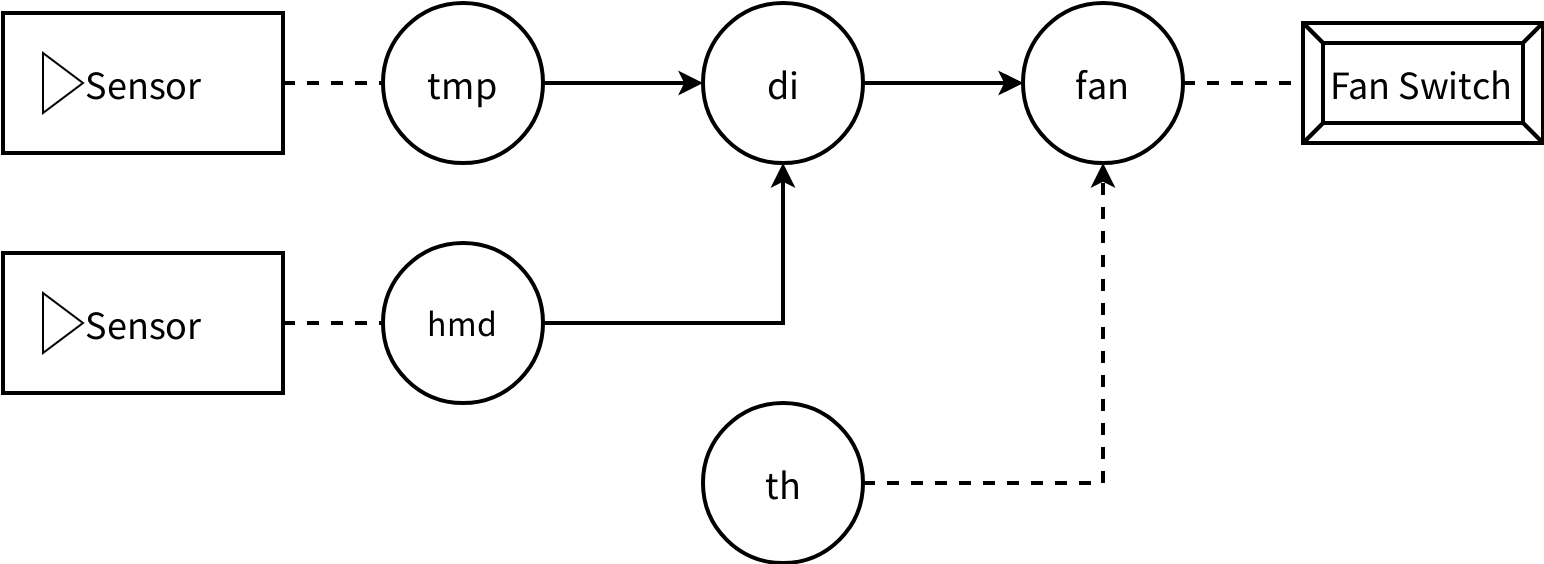
\includegraphics[scale=0.25]{./image/FanController.png}
                \end{center}
            \end{column}
            \begin{column}{0.55\textwidth}
                \vskip -0.4cm
                \begin{itemize}
                    \item Emfrpのプログラムは,時変値をノードとし依存関係を辺とした有向非巡回グラフ(DAG)を構成する.
                    \item 現在のEmfrpの処理系ではノードの更新は逐次的に行われる.左に挙げた例の場合,DAGをトポロジカルソートしたtmp$\rightarrow$hmd$\rightarrow$di$\rightarrow$th$\rightarrow$fanの順に更新が行われる.この更新(サイクル)を繰り返すことでリアクティブな動作を実現している.
                    \item 1サイクルにかかる時間がシステムの応答性を決める.本研究では,マルチコアシステムでの応答性向上を目的とした並列化方式を提案する.実行環境として汎用的なOSだけでなく,OSのない環境やFreeRTOS程度の小規模RTOSを考える.
                    \item 本研究の想定環境にはOSによるスケジューラによる適切なスケジューリングが期待できない環境も含まれている.そのため,実行モデルを並列化する際に実行モデルはOSのスケジューラに依存しないで動作する必要がある.
                    \item 本研究では,各サイクルの計算時間を短縮し,可能であれば応答時間を予測できるような静的スケジューリング方式を提案する.
                \end{itemize}
            \end{column}
        \end{columns}
    \end{block}

    \begin{block}{並列化アルゴリズム}
        \vskip 0.25cm
        本研究が提案するアルゴリズムはコンパイル時に静的にスケジューリングする.
        ただし,コンパイル時に使用するスレッド数は決定されていることを前提とする.
        下の図は実験で用いたアプリケーションを表現するグラフの一部であり,これを例とする.
        \begin{columns}
            \begin{column}{0.665\textwidth}
                提案する並列化アルゴリズムは各ノードから最も遠い到達可能なsinkノードへの距離を基準にスケジューリングを行う.
                ここでsinkノードとはグラフで出自数が0のノードであり,右の例ではノード$e_1,e_2$が相当する.
                グラフのノードの右上の数字が最も遠い到達可能なsinkノードへの距離である.
                並列化はこの最も遠い到達可能なsinkノードへの距離が等しいノードを並列に実行することで実現される.
                例えば,右のグラフのノード$a_1,a_2$は等しく距離3なので同時に実行可能,ノード$c_1,d_1,c_2,d_2$は等しく距離1なので同時に実行可能となる.
                同時に実行可能なノードの数が$N$個のとき,$M$スレッドで処理を行うならば1スレッドあたり$N/M$個のノードを更新すればよい.
                例えば2スレッドで右図を処理するならば,最長距離1のノードを更新する際は1スレッドあたり2つのノードを更新すれば良いのでスレッド1が$c_1,d_1$を,スレッド2が$c_2,d_2$を更新するというように更新する時変値を割り当てれば良い.
                %\begin{enumerate}
                %    \item 各ノードからsinkノードへの最長距離を計算する.ただし,sinkノードはグラフにおける出自数が0のノードである.
                %    \begin{itemize}
                %        \item グラフのノードの右上の数字はsinkノードへの最長距離
                %    \end{itemize}
                %    \item 同じ距離にあるノードを並列に更新する.
                %        \begin{itemize}
                %            \item OSのスケジューラを利用できない環境ではそれぞれのノードをどのプロセッサが更新するかを指定する必要がある.
                %            \item これは各スレッドがなるべく同じ数になるように割り当てる.
                %                \begin{itemize}
                %                    \item 下の表のsinkノードへの距離0のノード$3,5,7,8,9$を2スレッドで処理するならば$3,5$をスレッド1が$7,8,9$をスレッド2が更新.
                %                \end{itemize}
                %        \end{itemize}
                %\end{enumerate}
                \vskip-0.3cm
            \end{column}
            \begin{column}{0.3\textwidth}
                \begin{center}
                    \vskip-0.8cm
                    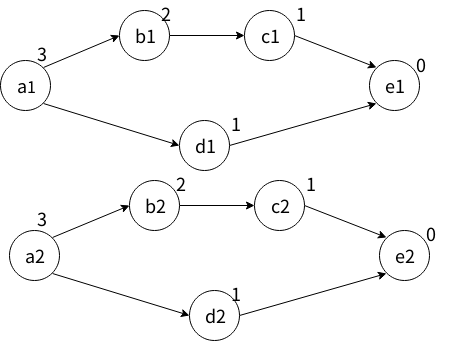
\includegraphics[scale=0.4]{image/lifegame.png}
                \end{center}
            \end{column}
        \end{columns}
        %\vskip-.7cm
    \end{block}

    \begin{block}{実験}
        \vskip 0.2cm
            提案する並列化アルゴリズムの性能を評価するために,XFRP-Core上で提案する実行モデルとEmfrpの実行モデルを実装し,$10^5$サイクルにかかる時間を測定した.
            実験は,Core i7-975上のUbuntu12.04で行った.
            並列化にはPthreadを使用し,同期にはPthreadライブラリで実装されているバリア同期を使用した.
            実験ではEmfrpの実行モデルは1スレッドで実行し,XFRP-Coreは2スレッドと4スレッドでそれぞれ10回計測し,その平均時間を実験結果とした.
            実験対象のアプリケーションとして,LifeGameと熱拡散シュミレータをXFRP上で実装した.
            アプリケーションで使用される時変値の数はそれぞれ$5\times10^5$個と$3\times10^5$個となった.
            実験結果は以下の表のようになった.
        \begin{columns}
            \begin{column}{0.55\textwidth}
                \vskip -0.3cm
                \begin{table}
                    \begin{tabular}{|l|c|r|r|} \hline
                        アプリケーション & Emfrp & XFRP-Core(2) & XFRP-Core(4) \\ \hline
                        LifeGame & 203.61(sec) & 108.04(sec) & 64.05(sec) \\ \hline
                        熱拡散シュミレータ & 65.70(sec) & 37.09(sec) & 25.88(sec) \\ \hline
                    \end{tabular}
                \end{table}
            \end{column}
            \begin{column}{0.4\textwidth}
                %\vskip -3.2cm
                LifeGameについては,XFRP-Coreの実行モデルで2スレッドと4スレッドを使用したときの実行時間はEmfrpの実行モデルの場合と比べてそれぞれ53.0\%と31\%になった.
                また,熱拡散シュミレータに対してはそれぞれ56.5\%,39\%の実行時間になった.
            \end{column}
        \end{columns} 
        \vskip -0.2cm
    \end{block}
\end{frame}
\end{document}
